%% Other market regimes and the out-of-sample window. Numbers from code/results/bench_{covid,bear2022,oos2026}.
\subsection{\blt{Other Market Regimes and an Out-of-Sample Window}} \label{s:regimes}
The 2023--2025 test period is a bull market. Table~\ref{tab:regimes} repeats the comparison, with the same universe, protocol, hyperparameters and 100 random portfolios per window, on three further 500-day windows: 2019--2020, which contains the COVID crash; 2021--2022, which contains the 2022 bear market; and September 2024 to September 2026, which lies almost entirely after the data used to design and tune the method and contains the live-test period of Sec.~\ref{s:live}. The 2019--2022 windows use the prices of the same 20 stocks before the 2021 screen that selected them, so they carry the selection bias of that screen (the stocks were chosen because they did well in 2021); the 2024--2026 window is free of it.

Three facts are stable across all four windows. (i) The corrected Risk-Averse policy has a lower Sharpe ratio than the rebalanced equal-weight portfolio in every window ($-0.2$ to $-0.8$, $p<0.001$), for the same reason as in Sec.~\ref{s:results}: it pays $11$--$15\%$ of its wealth in transaction costs per window. (ii) The legacy heuristic is the equal-weight portfolio plus $1\%$ of extra turnover: its Sharpe ratio is $0.02$ below that of the rebalanced equal-weight portfolio in every window, with a win rate of at most $4\%$. (iii) Against mean-variance the picture reverses with the regime: mean-variance made $4$--$7\times$ in 2019--2020 on the momentum of a few stocks and lost money in 2021--2022, whereas the Risk-Averse policy has a smaller drawdown than the 250-day mean-variance portfolio in $76$--$96\%$ of the portfolios in every window and a higher Sharpe ratio in the bear market ($+0.78$, $p<0.001$). In 2021--2022 both versions of the policy also beat the S\&P~500 in Sharpe ratio ($+0.53$ and $+0.72$), as does every low-turnover strategy on this universe; in the other windows the index is better. The out-of-sample window confirms the 2023--2025 ranking with no free parameter: equal-weight $1.06$, inverse volatility $0.91$, Risk-Averse $0.53$, S\&P~500 $1.16$.

\begin{table*}[ht!]
\centering
\footnotesize
\setlength{\tabcolsep}{4pt}
\begin{tabular}{lrrrrrrrrrrrr}
\hline
strategy & \multicolumn{3}{c}{2019-01 -- 2020-12} & \multicolumn{3}{c}{2021-01 -- 2022-12} & \multicolumn{3}{c}{2023-11 -- 2025-10} & \multicolumn{3}{c}{2024-09 -- 2026-09} \\
 & Sharpe & max DD & return & Sharpe & max DD & return & Sharpe & max DD & return & Sharpe & max DD & return \\
\hline
Risk-Averse (RA) & 0.71 & -40\% & 1.39 & 0.77 & -28\% & 1.37 & 0.34 & -25\% & 1.11 & 0.53 & -23\% & 1.20 \\
RA, legacy softmax solver & 1.46$^{*}$ & -37\% & 2.27 & 0.96$^{*}$ & -23\% & 1.55 & 0.63$^{*}$ & -27\% & 1.26 & 1.04$^{*}$ & -25\% & 1.55 \\
Equal-weight, rebalanced & 1.48$^{*}$ & -36\% & 2.29 & 0.98$^{*}$ & -23\% & 1.56 & 0.66$^{*}$ & -27\% & 1.27 & 1.06$^{*}$ & -25\% & 1.56 \\
Equal-weight, buy \& hold & 1.79$^{*}$ & -41\% & 3.75 & 0.92$^{*}$ & -23\% & 1.51 & 0.77$^{*}$ & -29\% & 1.36 & 1.01$^{*}$ & -26\% & 1.55 \\
Inverse volatility (60d) & 1.37$^{*}$ & -35\% & 1.99 & 1.06$^{*}$ & -23\% & 1.57 & 0.55$^{*}$ & -26\% & 1.20 & 0.91$^{*}$ & -25\% & 1.39 \\
Min-variance (250d) & 1.17$^{*}$ & -33\% & 1.70 & 1.01$^{*}$ & -24\% & 1.47 & 0.56$^{*}$ & -23\% & 1.18 & 0.67$^{*}$ & -21\% & 1.24 \\
Mean-variance (250d) & 1.66$^{*}$ & -44\% & 4.66 & -0.01$^{*}$ & -37\% & 0.90 & 0.69$^{*}$ & -40\% & 1.57 & 0.83$^{*}$ & -35\% & 1.85 \\
S\&P 500 (SPY) buy \& hold & 0.93$^{*}$ & -34\% & 1.49 & 0.23$^{*}$ & -24\% & 1.05 & 1.58$^{*}$ & -19\% & 1.62 & 1.16$^{*}$ & -19\% & 1.42 \\
\hline
\end{tabular}
\caption{Mean annualised Sharpe ratio, maximum drawdown and total return over 100 random portfolios (200 for the paper window) in four 500-day test windows: 2019--2020 contains the COVID crash, 2021--2022 the 2022 bear market, 2023--2025 is the window of the previous sections, 2024--2026 lies after the paper's data. Each window uses its own 250-day warm-up. $^{*}$: Sharpe ratio differs from that of the Risk-Averse policy at $p<0.01$ (paired Wilcoxon).}
\label{tab:regimes}
\end{table*}


\subsection{Live Test} \label{s:live}
\bl{We traded the policy with real money from 1 March to 15 April 2026 on a three-stock portfolio (Figs.~\ref{fig:cum_wealth_live}, \ref{fig:allocation_live}, Table~\ref{tab:live_metrics}). Over 32 trading days the policy returned $2.3\%$ against $2.2\%$ for the S\&P~500 and $5.6\%$ for the equal-weight portfolio, with the largest drawdown of the three. We keep the test because it demonstrates that the pipeline runs end-to-end on a broker feed, not as evidence of performance: 32 days cannot separate strategies whose daily returns differ by a fraction of a percent, and the 2024--2026 window above, which contains these dates, gives the same ranking on 100 portfolios.}


%% figures/table carried over verbatim from the previous version of the section
\begin{figure}[ht!]
    \begin{minipage}{0.45\textwidth}
    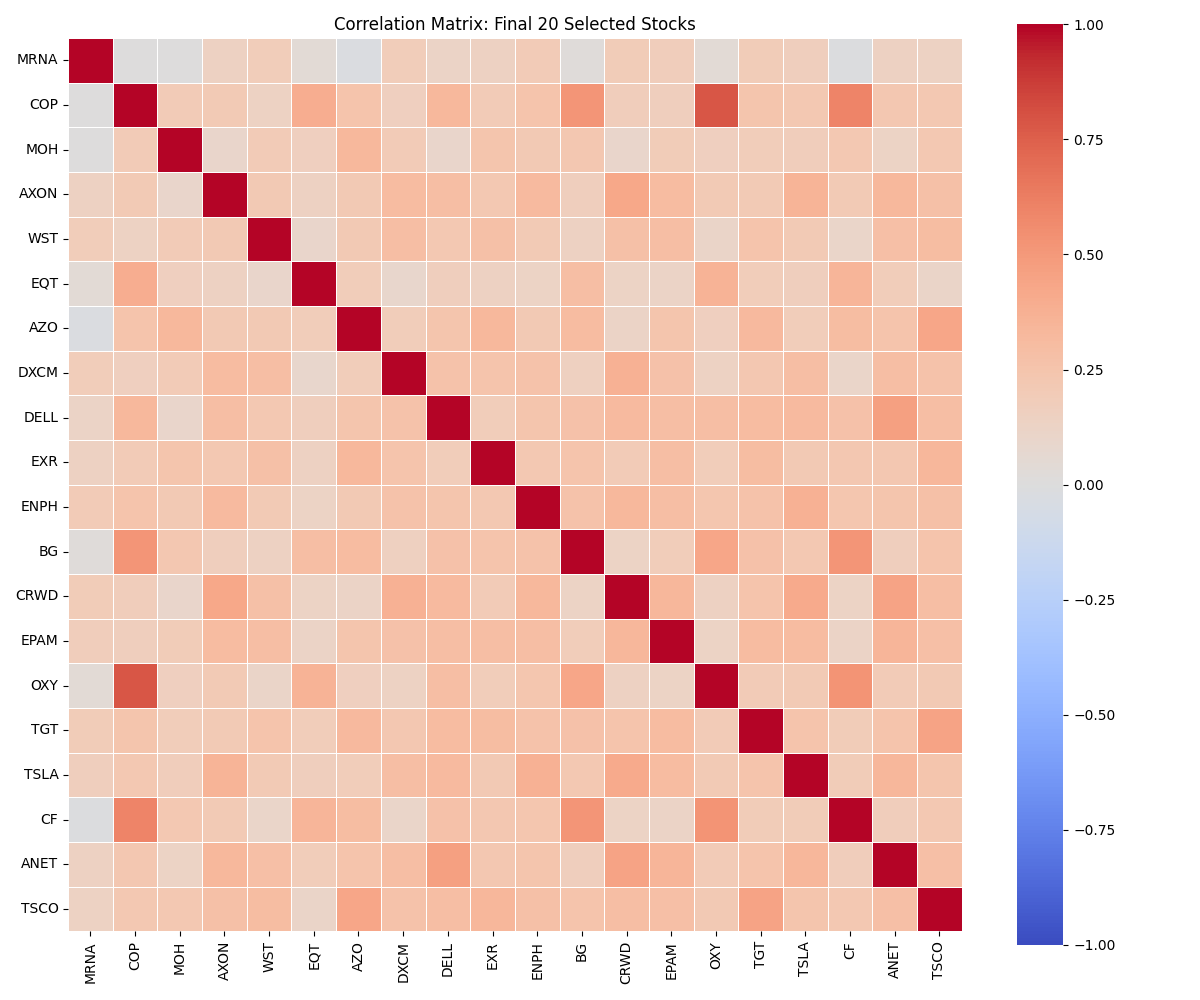
\includegraphics[width=\linewidth]{Images/selected_corr_matrix.png}
    \caption{Correlation matrix of the 20 selected stocks for our experiments.}
    \label{fig:corr_matrix}
    \end{minipage}
\end{figure}

\begin{figure}[ht!]
    \begin{minipage}{0.45\textwidth}
    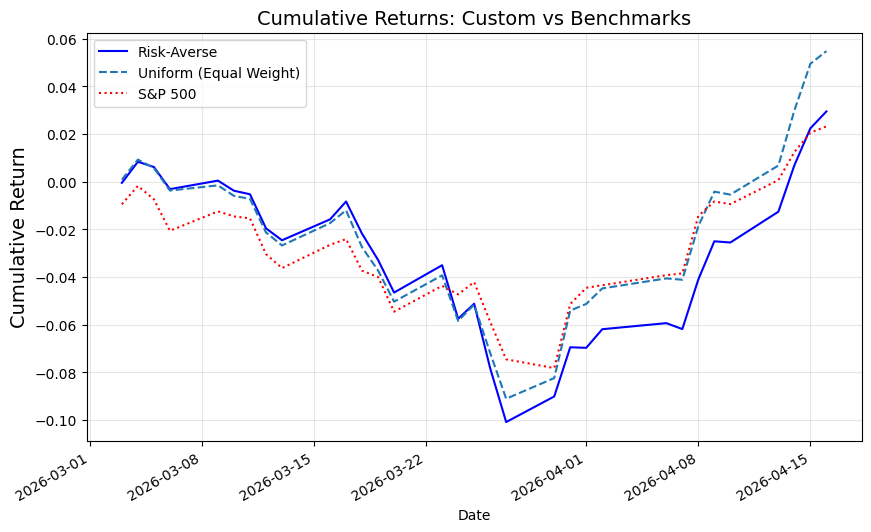
\includegraphics[width=\linewidth]{Images/live_returns.png}
    \caption{Returns comparison in live test. Risk Averse vs. Ideal Uniform portfolio vs. S\&P500 index benchmark.}
    \label{fig:cum_wealth_live}
    \end{minipage}
    \vfill

    \begin{minipage}{0.45\textwidth}
    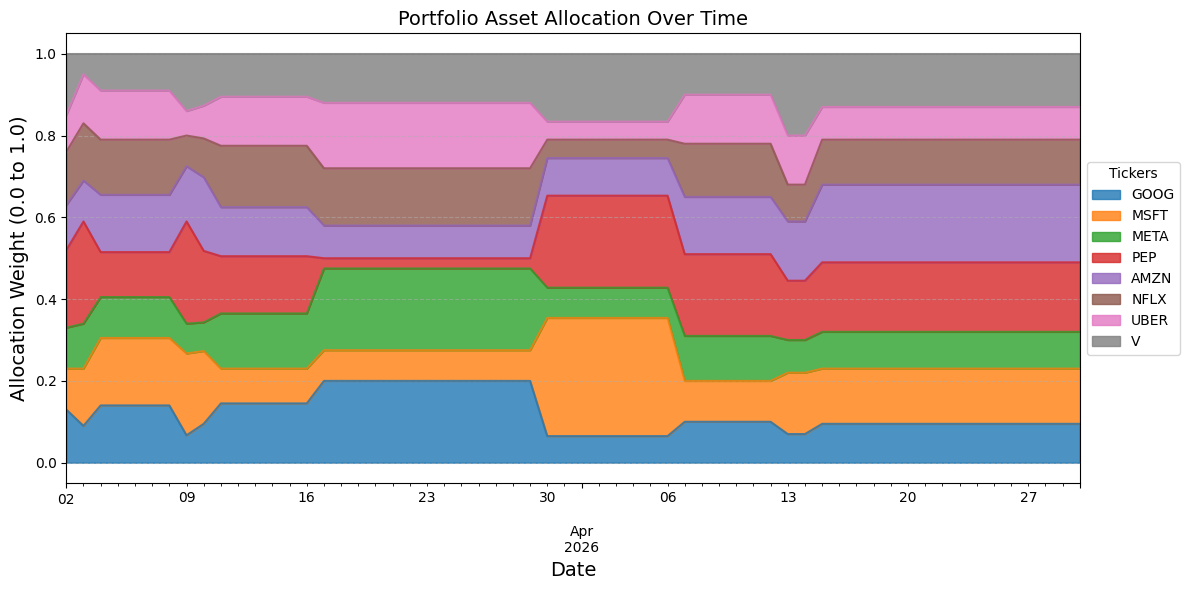
\includegraphics[width=\linewidth]{Images/live_allocation.png}
    \caption{Allocations of Risk Averse policy in live test.}
    \label{fig:allocation_live}
    \end{minipage}
\end{figure}

\begin{table}[ht!]
   \begin{minipage}{0.48\textwidth}
   % \centering
        \begin{tabular}{||l|r r r||} % Example table
        \hline
        & RA & U & S\&P500\\
        \hline
        max draw-down & -\textbf{0.108}& -0.099 & -0.077\\
        total return & \textbf{1.023} & 1.056 & 1.022\\
        SR & 0.074 & 0.133 & 0.069\\
        \hline
        \end{tabular}
      \caption{Comparison of live trading metrics.}
        \label{tab:live_metrics}
  \end{minipage}
\end{table}
